\section{Introduction}

\begin{figure}[h]
    \centering
    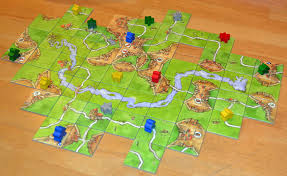
\includegraphics[width=0.5\textwidth]{images/Carcassonne.jpeg}
    \caption{(image tirée du site www.theboardgamefamily.com)}
    \label{fig:enter-label}
\end{figure}
%### Carcassonne : Un Classique Moderne des Jeux de Société

\subsection{Présentation générale du projet}
Carcassonne est un jeu de société moderne qui a su captiver l'imagination des joueurs depuis sa sortie en 2000. Créé par Klaus-Jürgen Wrede et édité par Hans im Glück, ce jeu tire son nom de la célèbre cité médiévale fortifiée située dans le sud de la France. Avec ses règles simples mais stratégiquement profondes, Carcassonne est devenu un pilier incontournable des soirées jeux de société à travers le monde.

\subsection{Principe du Jeu}
Le principe de Carcassonne est de construire un paysage médiéval en posant des tuiles représentant des villes, des routes, des champs et des abbayes. Chaque joueur dispose de partisans, aussi appelés meeples, qu'ils peuvent placer sur les tuiles pour revendiquer des territoires et marquer des points. Le but est d'avoir le plus de points à la fin de la partie.

\subsection{Déroulement d'une Partie}
\begin{itemize}
    \item \textbf{Mise en Place} : Au début de la partie, une tuile de départ est placée au centre de la table. Les autres tuiles sont mélangées et placées en piles face cachée.
    \item \textbf{Tour de Jeu} : À son tour, un joueur pioche une tuile et doit la placer de manière à ce qu'elle se connecte logiquement aux tuiles déjà en jeu. Par exemple, une route doit se connecter à une autre route, une ville à une autre ville, etc.
    \item \textbf{Placement des Meeples} : Après avoir placé une tuile, le joueur peut choisir de placer un meeple sur l'un des éléments de la tuile (ville, route, abbaye ou champ). Le meeple reste sur cette tuile jusqu'à ce que l'élément soit complété (comme la clôture d'une ville ou la fin d'une route).
    \item \textbf{Comptage des Points} : Une fois qu'un élément est complété, le joueur récupère son meeple et marque des points selon la taille de l'élément. Les champs, quant à eux, sont évalués à la fin de la partie.
\end{itemize}




%#### Stratégies et Complexité
Bien que Carcassonne soit facile à apprendre, il offre une profondeur stratégique surprenante. Les joueurs doivent constamment évaluer les risques et les récompenses de chaque placement de tuile et de meeple. Doivent-ils essayer de compléter leurs propres villes ou routes, ou gêner les autres joueurs ? Le positionnement des champs peut également être crucial, offrant des points supplémentaires en fin de partie pour chaque ville adjacente.
\subsection{Arborescence du dépot}
\begin{itemize}
    \item build :    \%contient tous les fichiers objets
    \item install
    \begin{itemize}
        \item all tests : \% l'exécutable des tests.
        \item server    : \% l'exécutable de la partie de jeu
        \item libplayer1.so : \% la bibliothèque dynamique du premier joueur.
        \item libplayer2.so : \% la bibliothèque dynamique du deuxième joueur.      
    \end{itemize}
    \item src : \% contient les codes sources sans les tests
    \begin{itemize}
        \item players : \% contient les deux fichiers sources des deux joueurs.
        \begin{itemize}
            \item player1.c 
            \item player2.c
        \end{itemize}
        \item les fichiers sources et d'en-têtes comme board.c board.h
    \end{itemize}
    \item tst : \% contient tous les fichiers sources pour les tests
    \item Makefile : \% compile l'ensemble des fichiers ainsi que les bibliothèques dynamiques des joueurs .
    \item README : \% contient des lignes d'explication afin de pouvoir compiler et exécuter les codes .
    \item .gitignore :  \% ignore les fichiers temporaires par git.
\end{itemize}
\subsection{Architecture du code}
Le projet est composé d’un ensemble de fichiers rédigés en langage de programmation C. Il comprend trois catégories de fichiers : les fichiers sources portant
l’extension ”.c” ,les fichiers d’en-tête portant l’extension ”.h” et les bibliothèques dynamiques poartant l'extension ".so". Les fichiers sources sont dédiés à la mise en œuvre du code, tandis que les fichiers d’en-tête servent à stocker les fonctions écrites dans les fichiers sources. Ils définissent également des variables globales en utilisant define, ainsi qu'un tableau \textbf{TILES\_TYPE} à l’aide de ”extern”.Chaque fichier fait les ”include” nécessaire pour la compilation. Nous avons adopté un fichier Makefile qui crée un fichier objet pour chaque fichier source, puis compile l’ensemble des fichiers en deux exécutables nommés ”server” pour les fichiers sources dans le répertoire \textbf{src} et ”alltests” pour les tests dans le répertoire \textbf{tst}. le fichier Makefile est censé aussi de compliler les bibliothèques dynamiques des joueurs. Ces dernières ainsi que les deux exécutables sont placés dans le répetoire \textbf{install}. En ce qui concerne les tests, nous avons utilisé des instructions ”printf” et ”assert” pour effectuer autant de tests que possible pour chaque fonction, en prenant en compte des cas extrêmes,de plus on a utilisé l'outil de développement logiciel \textbf{gcov} pour mesurer la couverture des tests.
voici le graphe de dépendances des fichiers sources situés dans la racine du répertoire \textbf{src}:
\begin{figure}[h]
    \centering
    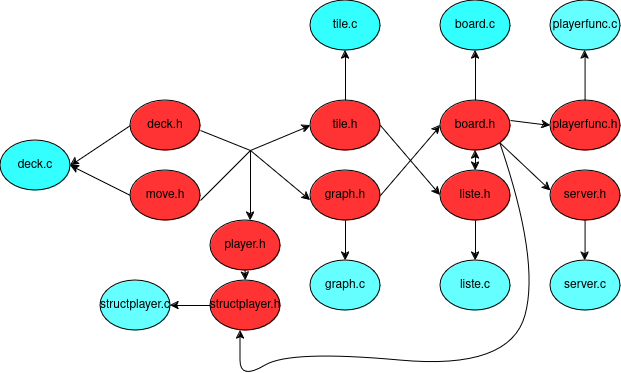
\includegraphics[width=0.9\textwidth]{images/Carcasonne.drawio(1).png}
    \caption{le graphe de dépendances des fichiers de \textbf{src} }
    \label{graphe de dépendaces}
\end{figure}
